\chapter{C/C++}
\label{sec:C/C++}
In der Vorlesung wurde mehr C als C++ gelehrt und gezielt auf fortgeschrittenen Konzepte wie Klassen, Exceptions, Templates, etc. verzichtet. 
\section{Basics}
\subsection{Variablen}\qquad\\
\begin{itemize}
	\item fängt mir a-z oder \_ an.
	\item enthält a-z, A-Z, 0-9,\_
	\item darf \textbf{nicht} mit einer Zahl beginnen. 
	\item enthalten Werte eines festen Typs.
	\item muss deklariert werden, bevor diese verwendet werden kann. Am besten direkt mit einem Startwert deklarieren.
	\item nach Konventionen, muss die Variable mit einem kleinen Buchstaben beginnen. 
\end{itemize}
\subsection{Arithmetische Operatoren}
\begin{itemize}
	\item + Addition
	\item += Addition mit Zuweisung
	\item - Subtraktion
	\item -= Subtraktion mit Zuweisung
	\item * Multiplikation
	\item *= Multiplikation mit Zuweisung
	\item / Division
	\item /= Division mit Zuweisung
	\item \% Modulo
\end{itemize}
\subsection{Increment / Decrement}
\begin{tabular}{ccc}
	& prefix & postfix \\ 
increment	& ++a & a++  \\ 
decrement	& --a & a-- \\ 
\end{tabular} \\\qquad \\
Der Unterschied zwischen prefix und postfix ist, dass bei einer Zuweisung wie
\begin{lstlisting}[language=C++] 
a = ++b;
\end{lstlisting}
der Wert von b erst erhöht wird und danach erst zugewiesen wird. Bei 
\begin{lstlisting}[language=C++] 
a = b++;
\end{lstlisting}
wird der Wert erst zugewiesen und daraufhin erhöht. 
\subsection{Typen}
\begin{figure}[h]
\centering
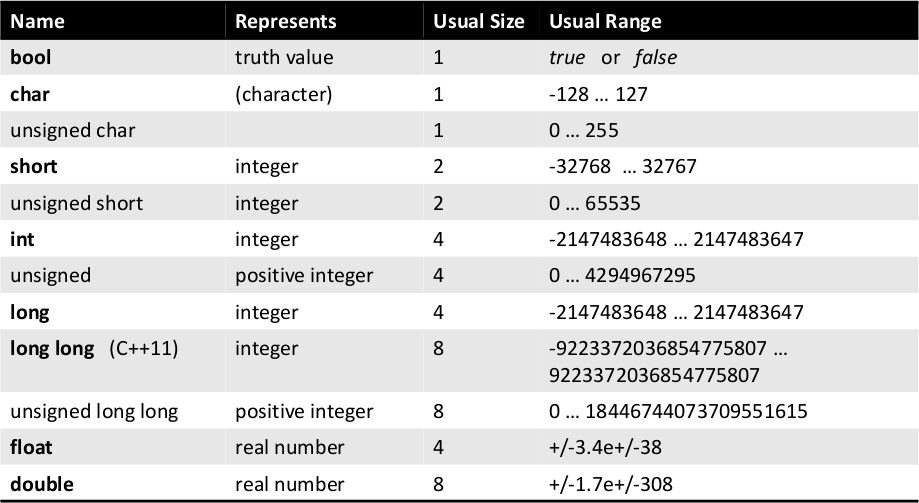
\includegraphics[width=0.75\linewidth]{mainmatter/pics/typ}
\caption[typen]{Alle Typen im Überblick}
\label{fig:typ}
\end{figure}
Jedoch gilt es zu beachten das long und int meist gleich lang sind auf 32Bit Systemen und das der C++ Standard lediglich die Minimale Größe Garantiert.
\subsection{Logik Operationen}\qquad\\
\&\& / and = Und\\
|| / or = Oder\\
! / not = Negation\\
0 = false\\
alles $\neq$ 0 = true
\subsection{Vergleiche}
== ; < ; > ; >=; <= ; !=
		
\subsection{Funktionen}
\begin{lstlisting}[language=C++]
return_type name (parameters) {
	//body
}
\end{lstlisting}
Die Main Funktion wird mit dem return\_type int versehen, da Programme in der Regel eine 0 zurückliefern, sofern diese ohne Probleme durchgelaufen sind. 
\section{Programme Kompilieren}
\subsection{C++ Programme bauen}\qquad\\
Ein Programm in C++ kann aus mehreren Header Dateien (*.h) und Quellcode Dateien (*.cpp) bestehen. Um diese zu einem Lauffähigen Programm umzuwandeln. Benötigt man einen Compiler wie g++. Dieser Besteht aus einem Linker, Preprocessor und dem Compiler selbst. \\
Der Preprocessor nimmt alle in den Sourcecode verlinkten Header Dateien und fügt diese zu 100 \% in den Sourcecode in dieser Stelle ein. Die Header Dateien können gleichzeitig in mehreren Sourcecode Dateien stecken. \\
Der Compiler wandelt anschließen die Sourcecode Dateien in Objectdateien um, welche vom Menschen nciht mehr gelesen werden können.\\
Der Linker fügt alle Object Dateien mit den verwendeten externen Bibiliotheken zu einem ausführbaren Programm zusammen. Dabei werden auch alle Sprungadressen für Funktionsaufrufe gesetzt\\
\begin{figure}[h]
\centering
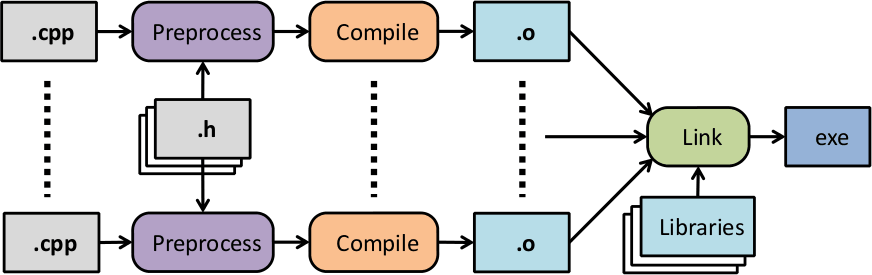
\includegraphics[width=0.75\linewidth]{mainmatter/pics/comp}
\caption[compiling]{C++ Programm Kompilieren}
\label{fig:comp}
\end{figure}
\subsubsection{Wozu dieses große Konstrukt?}
Viele Projekte enthalten eine sehr große Menge an Quellcode Dateien. Da man nicht bei jeder kleinen Änderung alle cpp Dateien neu in Objekt Dateien umwandeln will. Kann man auch schlicht nur die geänderten cpp Dateien durch den Preproccesor jagen und anschließend alle .o Dateien neu zu verlinken um die Änderungen zu testen. \\
Außerdem können vorhandene doppelte \#includes verhindert werden, indem man diese mit Guards definiert. Diese verhindern, dass die header Dateien, selbst bei mehrfacher Verlinkung, mehrfach in den Code einkopiert werden. \newpage
\begin{lstlisting}[language=C++]  
//Datei: foo.h
#ifndef A_H
#define A_H
struct foo {
	int member;
};
void f(foo&);
...
#endif
\end{lstlisting}
Selbst wenn man nun die foo.h header Datei in mehreren Dateien included, wird sie lediglich einmal hinzugefügt. Denn der Preprocessor, erkennt alle mit \# markierte Zeilen als seine an und führt das if entsprechend der Definition aus. Dabei geht der Guard von \#ifndef A\_H bis \#endif. Das \#define bedeutet, wenn A\_H noch nicht definiert wurde, definiere diese wie folgt. \\
\subsection{Wie lauten die Terminal Befehle dafür?} 
Die Terminal Befehle lauten wie folgt. 
\begin{lstlisting}[language=bash]
g++ -c source.cpp 
g++ -c dbl.cpp 
g++ source.o dbl.o -o test 
\end{lstlisting}
Mit dem Parameter -c werden die angegebenen cpp Dateien in Object Files umgewandelt. Danach linkt man die Object Files mit Hilfe des Parameters -o. Man kann auch direkt -o verwenden wenn man die Dateien direkt in eine .exe Datei umwandeln will.\\
Um das Kompilieren zu vereinfachen, benutzt man bei vielen Dateien eine Makefile. Einen solche sieht wir folgt aus. 
\begin{lstlisting}[language=bash]
#name test
#comment
#compile main 
main.o : main.cpp 
	g++ -c main.cpp 
#compile other 
other.o : other.cpp 
	g++ -c other.cpp 
#link 
prog: main.o other.o 
	g++ main.o other.o -o prog 
\end{lstlisting}
Der Aufruf der Makefile läuft folgendermaßen
\begin{lstlisting}[language=bash]
make test
./prog 
\end{lstlisting}
Mit ./ führt man die generierte .exe aus. 
\section{Kommandozeilen Argumente}
Hier ein kleines Beispiel, wie man Kommandozeilen Argumente beim Start eines Programmes direkt übergibt, ausliest und auf der Konsole ausgibt. 
\begin{lstlisting}[language=C++]
#include <iostream>

using namespace standard

int main(int argc, char* argv[])
{
for(int i = 1; i<argc;++i){
cout << argv[i] <<endl;
}
return 0;
}
\end{lstlisting}
\begin{lstlisting}[language=Bash]
> ./test 12 3 abc def
test
12
3
abc
def
\end{lstlisting}
argc und argv sind nur Konventionen und können anders benannt sein. argc enthält die Anzahl der Elemente und argv ist ein C Array. Die Elemente von argv sind wiederum C Strings.  
\section{I/O from console/file}	\qquad\\

\section{Control Statements and Loops}
\subsection{if .. then .. else / Switch}
\begin{lstlisting}[language=C++]
if (condition1) {
	//do this if condition1 is true
}
else if (condition2) {
	//otherwise do this if
	//condition2 is true
}
else {
	//otherwise do this 
}
\end{lstlisting}
\qquad\\
\begin{lstlisting}[language = C++]
switch(m){
	case 0:
		//do this if 0
		break;
	case 1:
		//do this if 1 and got to the next 
		//cause of missing break
	case 3: 
		//do this if 3
	break;
	default:
		// if everything else fails do this	
}
\end{lstlisting}
Für das m im switch können char, int, long und weitere Zahlenwerte verwendet werden. 

\subsection{Loops}
\begin{lstlisting}[language=C++]
for (int i = 0; i < 5; ++i) {
cout << i << endl;
}

int j = 5;
while (j < 10) {
cout << j << endl;
++j;
}

do {
cout << j << endl;
--j;
} while (j > 0);
\end{lstlisting}	
\section{Call by Value / Call by Reference}
\section{Pointer und Referenzen}
\subsection{Referenzen}
Referenzen referenzieren einen Wert lediglich. Wenn man den Wert einer Referenz ändert, so ändert man den Wert der Variable auf den die Referenz zeigt. Dies ist nützliche, da man Werte als Referenzen an eine Methode übergeben kann. Dadurch hat man die Möglichkeit sich mehr als einen return Wert zu generieren. Da man die Variable außerhalb der Methode ändert und nicht nur die Unbekannte innerhalb der Methode. \\
\begin{lstlisting}[language=C++]
// Initialisierung
int i = 2;
int& ri = i; 
const int& ci = i;
double& blub = i; // => Fehler da die Typen identisch sein muessen.
int& rj; // Fehler, da Referenzen immer initialisiert sein muessen

// Wertzuweisung

\end{lstlisting}
\section{Memmory Management (Stack/Freestore)}
\section{Structs}
\section{Complex Data Structures (Lists, Trees)}
\section{Standard Containers and Algorithms}	

